\section{Problem definition}
With the advancements of technology,
people tried digitalizing every aspect of their life.
They renounced the traditional slow postal services in favour of
the modern fast email.
Digital photos gained popularity to the detriment of physical copies.
In the same way, CD-s and other physical mediums were
forgotten with arising of digital MP3s.

Over the past years, with the rise of the internet,
from digitalizing their lives, people started to sync
it with the cloud. Hence, a new way of storing and
transmitting data emerged: streaming.

\begin{figure}[h]
      \centering
      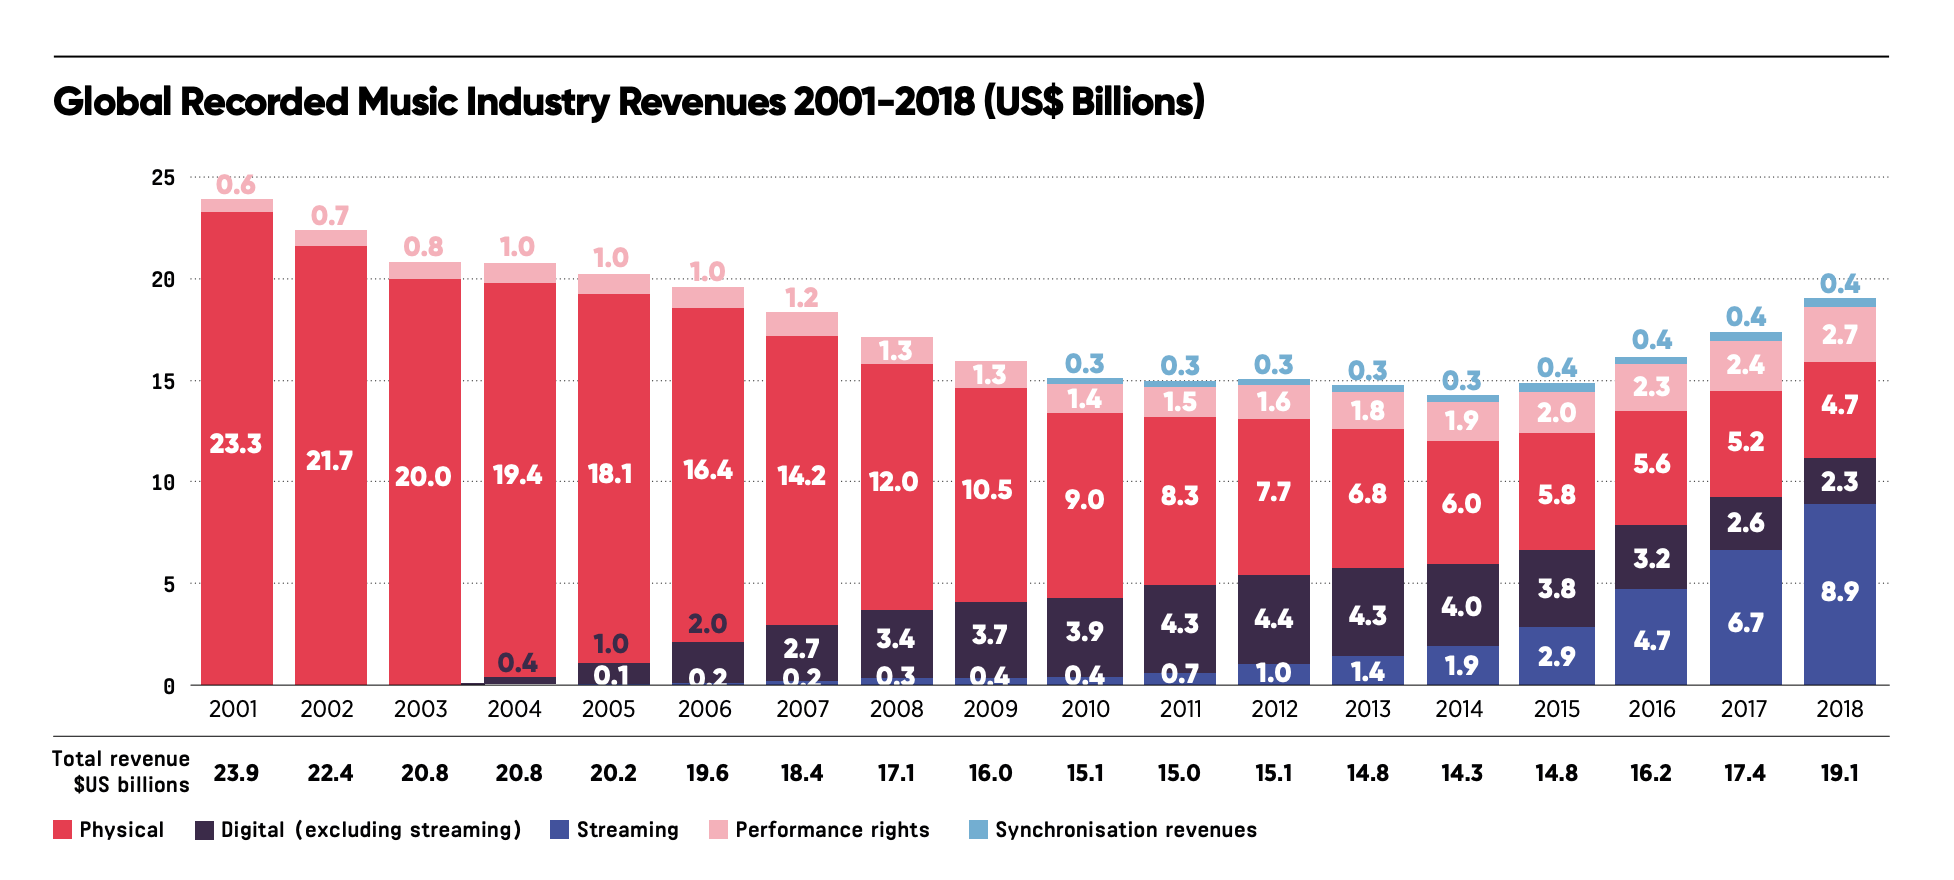
\includegraphics[width=1\textwidth]{ifpi}
      \caption{\emph{Global Recorded Music Industry Revenues 2001-2018  \cite{ifpi}}}
      \label{fig:ifpi}
\end{figure}

As depicted in  Figure\emph{~\ref{fig:ifpi}}, in the last decade,
the revenue of the musing industry shifted,
going from physical to digital, in the end,
the highest revenue being generated by streaming means.

With this change, one can easily compose and produce
music from their studio or even bedroom,
since it is not compulsory to be tied to a record label.
There are lots of successful independent musicians who
create music in this way and the numbers are growing more
and more every year \cite{forbes}.

Even with all these developments,
the act of composing music did not drastically change in the last
few hundred years. If one wants to compose a song,
they should learn how to use instruments,
and how to put notes in such a manner that they sound good together.
Technology eased the process of composing,
but one must still learn chords, scales,
and other elements of music theory to make the process less hazardous.
Although music theory has a steep learning curve,
learning it helps express oneself musically.
Despite all these advancements,
there is a lack of tools facilitating the creative process.

\section{Functional requirements}
This section contains details about the functional requirements
of the application and its main purpose,
composing music based on feelings.

The application software allows the user to
input arousal and valence values and to tweak other
features that our model learned, and it should generate a song.

Bellow, there is a list of the main features the app has:
\begin{itemize}[]
      \item
            The user should be able to input values for valence and arousal and the app should respond with a composed song based on them
      \item
            The user should be able to listen to the generated song
      \item
            The user should be able to change the instrument in which the song is rendered
      \item
            It should be capable of modifying the input and see live edits of the displayed song
      \item
            The app should allow the user to export the file as MIDI and save it to its computer
\end{itemize}
% \begin{table}[]
%     \begin{tabular}{ll}
%         \hline
%         No crt & Requirement                                                                                                                    \\ \hline
%         1      & The user should be able to input values for valence and arousal  and the app should respond with a composed song based on them \\
%         2      & The user should be able to listen to the generated song                                                                        \\
%         3      & The user should be able to change the instrument in which the song is rendered                                                 \\
%         4      & It should be capable of modifying the input and see live edits of the displayed song                                           \\
%         5      & The app should allow the user to export the file as MIDI and save it to its computer
%     \end{tabular}
% \end{table}

% \section{Model Design}
% The model used in this thesis is created using Keras with Tensorflow as its backend.
% We have chosen this frameworks, so we can focus more on our data and how to explore it,
% and not on the implementation of some existing algorithms.

% \begin{figure}[h]
%       \centering
%       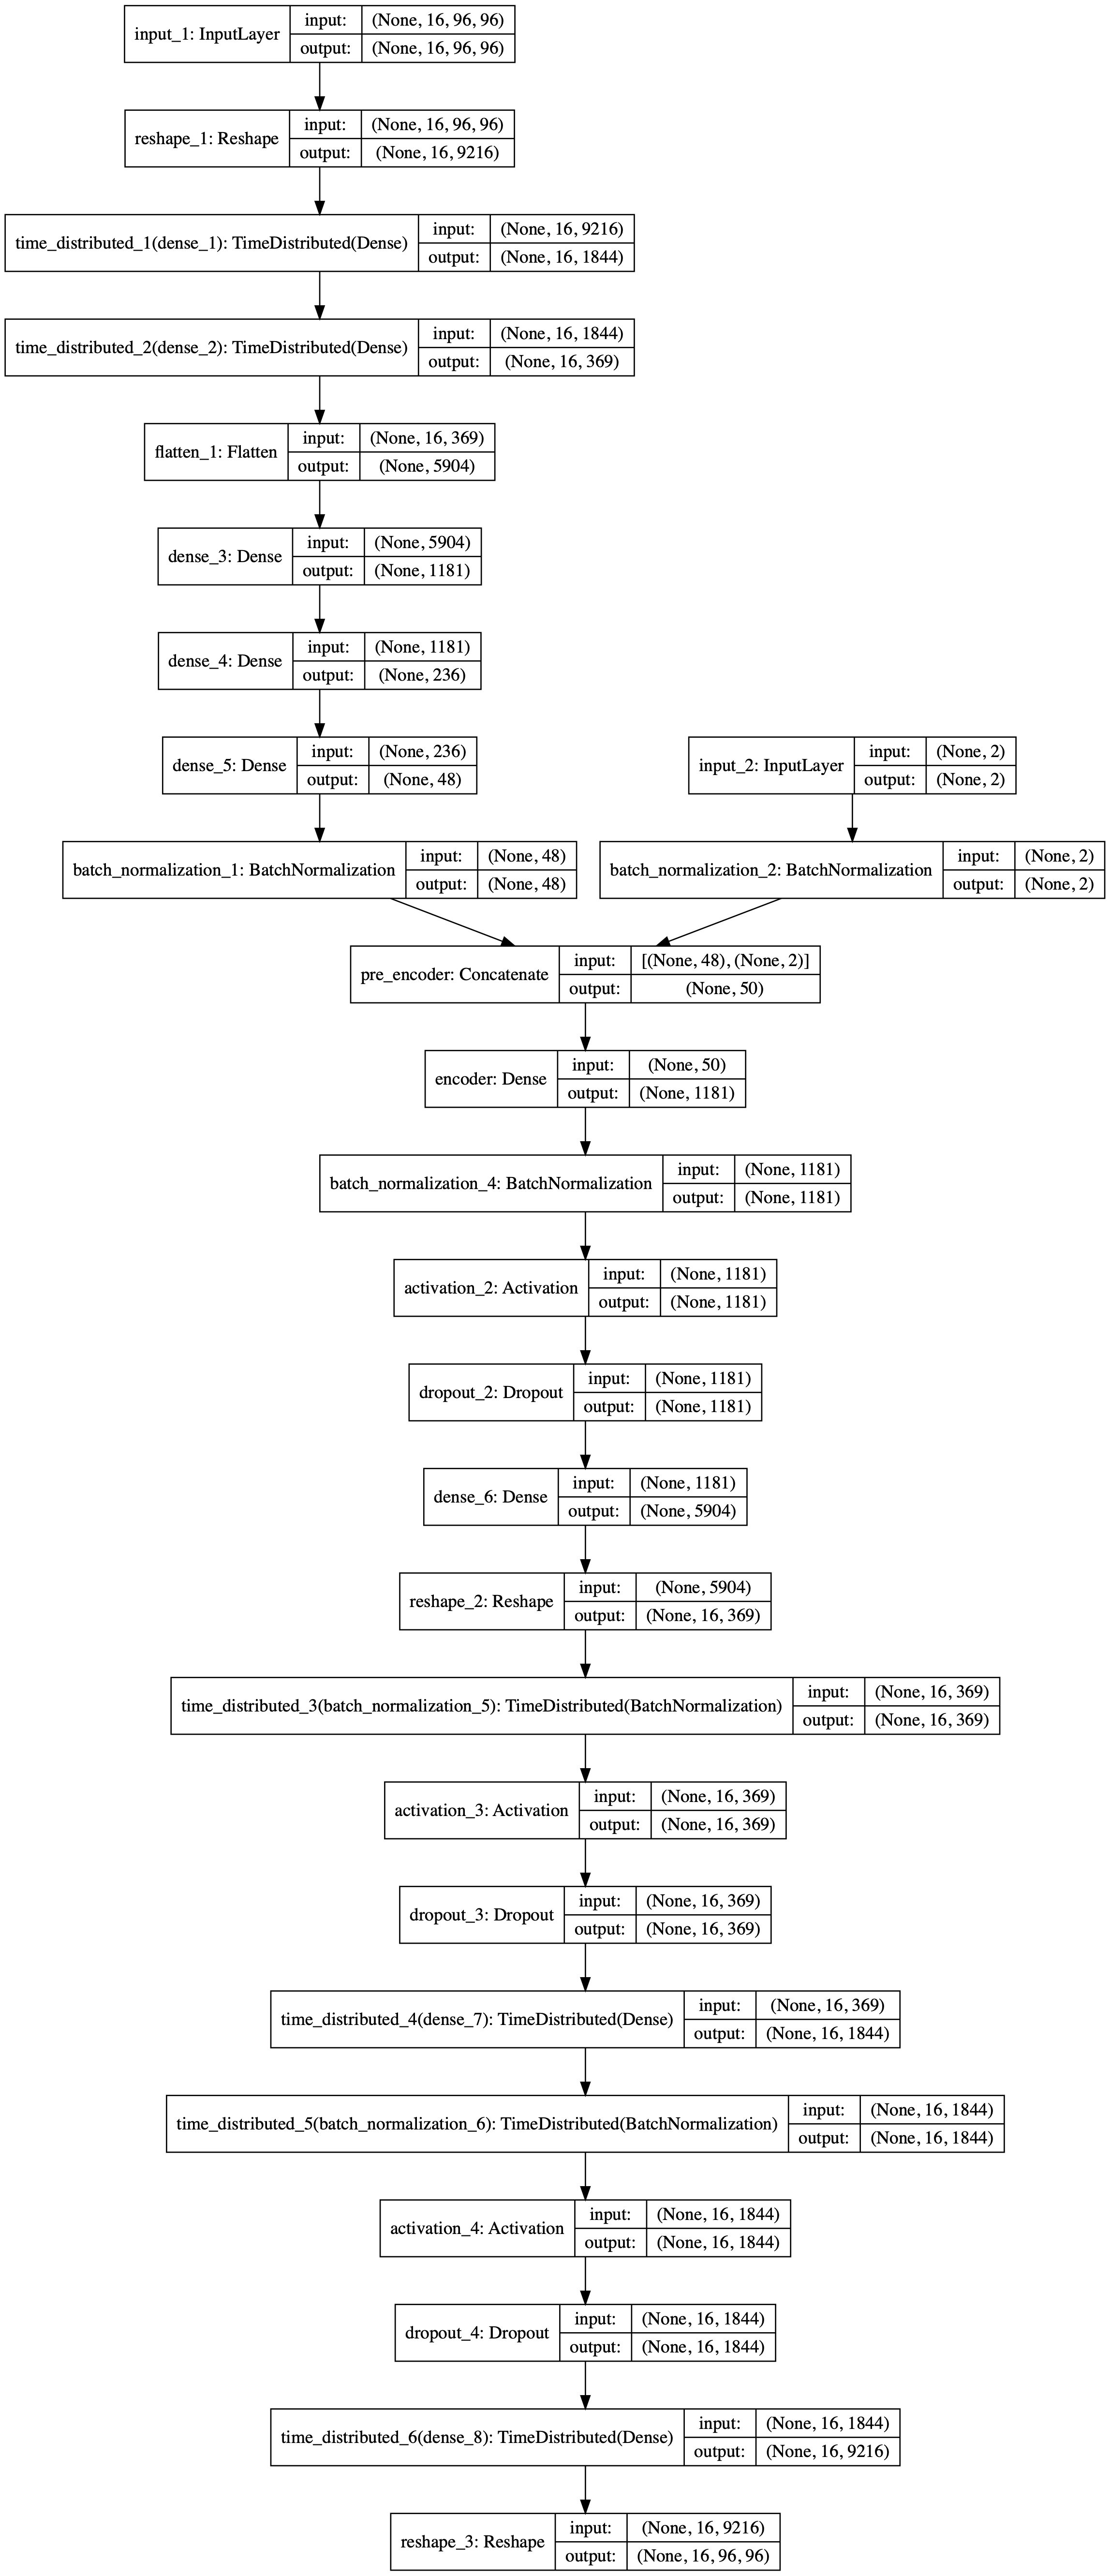
\includegraphics[width=0.75\textwidth]{model}
%       \caption{\emph{Structure of our main model}}
%       \label{fig:model}
% \end{figure}

% A graphical representation of the structure of the model can be seen in the Figure\emph{~\ref{fig:model}}
